\chapter{Contexte général du projet}


\cleardoublepage

\section{Présentation de l’OCP}
	\subsection{Historique}
	En 1920, alors que partout dans le monde, les compagnies minières fouillent fébrilement le
sous-sol à la recherche du phosphate, minerai aux précieuses vertus fertilisantes, l’Office
Chérifien des Phosphates (OCP S.A. depuis 2008) voit le jour.

En 1965, avec la mise en service du Maroc Chimie à Safi, le groupe devient également
exportateur de produits dérivés. En 1998, il franchit une nouvelle étape en lançant la fabrication
et l’exportation d’acide phosphorique purifié.

Parallèlement, de nombreux partenariats sont développés avec des opérateurs industriels du
secteur, au Maroc et à l’étranger.
	\subsection{Fiche signalétique}
	\begin{description}[align=left]
		\item [Nomination sociale :] Groupe Office Chérifien des Phosphates
		\item [Date de création :] 1920
		\item [Siège social :] 2-4, rue Al Abtal, Hay Erraha, 20200 Casablanca
		\item [Capital social :] 8287 M MAD (2013)
		\item [Effectif employé :] 23,000 (2013)
		\item [Site web :] www.ocpgroup.ma
	\end{description}
	\subsection{Quelques événements marquants de l’histoire du Groupe OCP}
	\begin{description}[align=left]
		\item [1920 :] Création, le 7 août, de l'office chérifien des Phosphates (OCP).
		\item [1959 :] Création de la société marocaine d'études spécialisées et industrielles (SMESI).
		\item [1965 :] Création de la société Maroc Chimie.
		\item [1974 :] Lancement des travaux pour la réalisation du centre minier de Benguérir, en mai.
		\item [1975 :] Création du Groupe OCP avec l'intégration des industries chimiques aux
		\item [1998 :] Le Groupe OCP obtient le Prix National de la Qualité.
		\item [2003 :] L'OCP est devenu le seul actionnaire de Phosboucraâ.
		\item [2008 :] La société anonyme OCP SA est née le 22 janvier - Démarrage de Pakistan Maroc
		\item [2009 :] Démarrage de Bunge Maroc Phosphore à Jorf Lasfar (BMP).
		\item [2010 :] Création de JESA, joint-venture sous forme de partenariat en ingénierie
		\item [2012 :] Creation de la JV BSFT (Black Sea Fertilizer Trading Company)
		\item [2013 :] Signature d’une joint-venture avec Dupont
		\item [2014 :] Inauguration du SLURRY PIPELINE entre Khouribga et Jorf Lasfar
	\end{description}
	
	\subsection{Filiales et Partenariats}
	L'OCP se structure en quatre filières chacune se focalisant sur un segment du groupe OCP et ayant co-creer plusieurs coentreprises dont la figure \ref{fig:mesh1} fait la liste : 
	\begin{figure}[h]
    		\centering
<<<<<<< HEAD
    		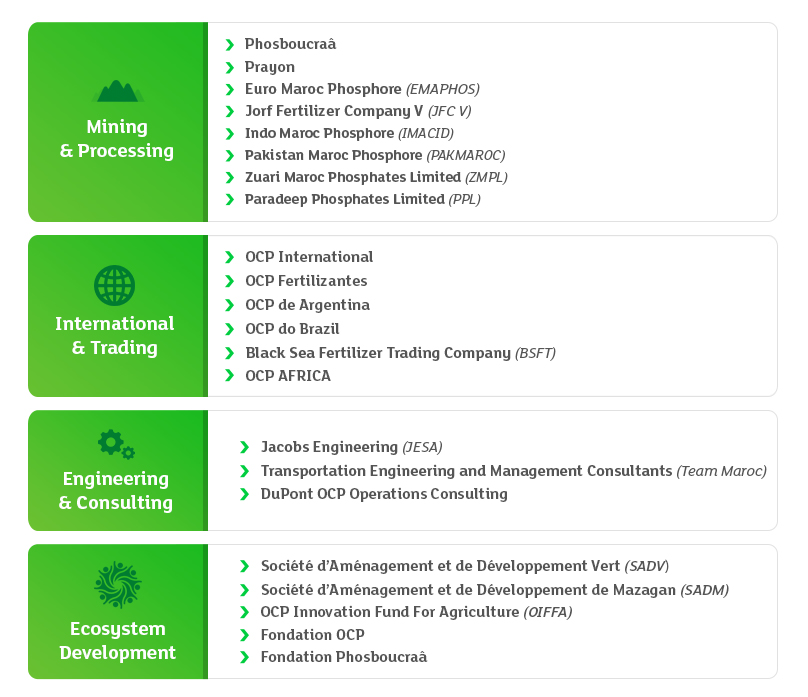
\includegraphics[scale=0.25]{Companies-ocp}
    		\caption{Filiales et Coentreprises de l’OCP}
=======
    		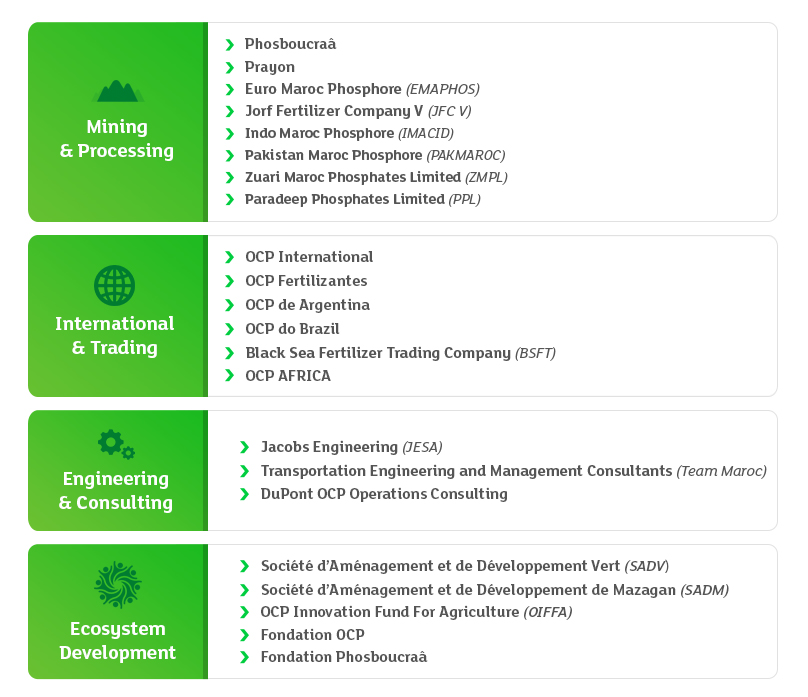
\includegraphics[scale=0.5]{Companies-ocp}
    		\caption{Filiales et Coentreprises de l’OCP\cite{ocp-fil}}
    		\label{fig:mesh1}
>>>>>>> 37a30d85365a259940e9c5fea7ebf670a9b69210
	\end{figure}
	
	
\section{Présentation du projet}
	\subsection{Cadre général du projet}
	
	\subsection{Motivation et Problématique}


\section{Planification du projet}
	\subsection{Les étapes CRISP-DM d'un projet Data Mining}
	\subsection{Le planning du projet}